\documentclass[12pt,a4paper]{article}
\usepackage[utf8]{inputenc}
\usepackage[spanish]{babel}
\usepackage[margin=0.5in, top=0.5in, bottom=0.5in]{geometry}
\usepackage{amsmath}
\usepackage{amsfonts}
\usepackage{amssymb}
\usepackage{hyperref}
\usepackage[shortlabels]{enumitem}
\usepackage{graphicx}
\newcommand{\p}{\phantom{......}}

\usepackage{setspace}
\onehalfspacing

\title{Bases de datos 2023-1\\
Tarea 4: Álgebra Relacional}
\begin{document}
\maketitle

\begin{enumerate}
	\item[1.] Cardinalidad de la consulta
		Considera las siguientes relaciones:\\

		\begin{minipage}{0.5\textwidth}
		\textbf{R}\\
		\begin{tabular}{|l|l|}
			\hline
			A	& B\\
			\hline
			1	& x\\
			2	& y\\
			2	& z\\
			3	& x\\
			9	& a\\
			\hline
		\end{tabular}
		\end{minipage}
		\begin{minipage}{0.5\textwidth}
		\textbf{S}\\
		\begin{tabular}{|l|l|l|}
			\hline
			B	& C	& D\\
			\hline
			x	& 0	& 3\\
			y	& 2	& 1\\
			y	& 3	& 3\\
			w	& 3	& 0\\
			y	& 4	& 2\\
			\hline
		\end{tabular}
		\end{minipage}

		Para las siguientes expresiones de álgebra relacional completa la tabla con el número de tuplas.
		Deberás indicar las tablas resultantes en cada caso.\\
		\begin{tabular}{|l|l|}
			\hline
			Expresión		& Cardinalidad del resultado\\
			\hline
			$R \times S$											& 25\\
			$R \bowtie_{\theta D > A} S$							& 7\\
			$R =\bowtie  S$											& 7\\
			$R \bowtie=  S$											& 6\\
			$R \bowtie_{\theta A=D} S$								& 5\\
			$\rho_{C \leftarrow A}(R) \bowtie S$					& 4\\
			$\Pi_B (R) - \Pi_B (\sigma_{C \geq 3} (S))$				& 3\\
			$\Pi_A (R) \cap \rho_{A \leftarrow D} (\Pi_D (S))$		& 3\\
			$\Pi_D (S) \bowtie R$									&20\\
			$\gamma_{A ; count(B) \rightarrow t} (R =\bowtie= S)$	&5\\
			\hline
		\end{tabular}

		\pagebreak
		\textbf{tablas}:
		\begin{itemize}
			\item $R \times S$\\
				\begin{tabular}{|l|l|l|l|l|}
					\hline
					A	&BR	&BS	&C	&D\\
					\hline
					1	&x	&x	&0	&3\\
					1	&x	&y	&2	&1\\
					1	&x	&y	&3	&3\\
					1	&x	&w	&3	&0\\
					1	&x	&y	&4	&2\\
					\hline
					2	&y	&x	&0	&3\\
					2	&y	&y	&2	&1\\
					2	&y	&y	&3	&3\\
					2	&y	&w	&3	&0\\
					2	&y	&y	&4	&2\\
					\hline
					2	&z	&x	&0	&3\\
					2	&z	&y	&2	&1\\
					2	&z	&y	&3	&3\\
					2	&z	&w	&3	&0\\
					2	&z	&y	&4	&2\\
					\hline
					3	&x	&x	&0	&3\\
					3	&x	&y	&2	&1\\
					3	&x	&y	&3	&3\\
					3	&x	&w	&3	&0\\
					3	&x	&y	&4	&2\\
					\hline
					9	&a	&x	&0	&3\\
					9	&a	&y	&2	&1\\
					9	&a	&y	&3	&3\\
					9	&a	&w	&3	&0\\
					9	&a	&y	&4	&2\\
					\hline
				\end{tabular}

			\item $R \bowtie_{\theta D > A} S$\\
				\begin{tabular}{|l|l|l|l|l|}
					\hline
					A	&BR	&BS	&C	&D\\
					\hline
					1	&x	&x	&0	&3\\
					1	&x	&y	&3	&3\\
					1	&x	&y	&4	&2\\
					\hline
					2	&y	&x	&0	&3\\
					2	&y	&y	&3	&3\\
					\hline
					2	&z	&x	&0	&3\\
					2	&z	&y	&3	&3\\
					\hline
				\end{tabular}

			\pagebreak
			\item $R =\bowtie  S$\\
				\begin{tabular}{|l|l|l|l|l|}
					\hline
					A	&BR	&BS	&C	&D\\
					\hline
					1	&x	&x		&0		&3\\
					2	&y	&y		&2		&1\\
					2	&y	&y		&3		&3\\
					2	&y	&y		&4		&2\\
					2	&z	&NULL	&NULL	&NULL\\
					3	&x	&x		&0		&3\\
					9	&a	&NULL	&NULL	&NULL\\
					\hline
				\end{tabular}

			\item $R \bowtie= S$\\
				\begin{tabular}{|l|l|l|l|l|}
					\hline
					A	&BR	&BS	&C	&D\\
					\hline
					1	&x	&x	&0	&3\\
					3	&x	&x	&0	&3\\
					2	&y	&y	&2	&1\\
					2	&y	&y	&3	&3\\
					NULL	&NULL	&w	&3	&0\\
					2	&y	&y	&4	&2\\
					\hline
				\end{tabular}

			\item $R \bowtie_{\theta A=D} S$\\
				\begin{tabular}{|l|l|l|l|l|}
					\hline
					A	&BR	&BS	&C	&D\\
					\hline
					1	&x	&y	&2	&1\\
					2	&y	&y	&4	&2\\
					2	&z	&y	&4	&2\\
					3	&x	&x	&0	&3\\
					3	&x	&y	&3	&3\\
					\hline
				\end{tabular}

			\item $\rho_{C \leftarrow A}(R) \bowtie S$\\
				\begin{tabular}{|l|l|l|l|}
					\hline
					C	&RB	&SB	&D\\
					\hline
					2	&y	&y	&1\\
					2	&z	&y	&1\\
					3	&x	&y	&3\\
					3	&x	&w	&0\\
					\hline
				\end{tabular}

			\item $\pi_B (R) - \pi_B (\sigma_{C \geq 3} (S))$\\
				\begin{tabular}{|l|}
					\hline
					B\\
					\hline
					x\\
					z\\
					a\\
					\hline
				\end{tabular}

			\item $\Pi_A (R) \cap \rho_{A \leftarrow D} (\Pi_D (S))$\\
				\begin{tabular}{|l|}
					\hline
					A\\
					\hline
					1\\
					2\\
					3\\
					\hline
				\end{tabular}

			\pagebreak
			\item $\Pi_D (S) \bowtie R$\\
				\begin{tabular}{|l|l|l|}
					\hline
					D	&A	&B\\
					\hline
					3	&1	&x\\
					1	&1	&x\\
					0	&1	&x\\
					2	&1	&x\\
					\hline
					3	&2	&y\\
					1	&2	&y\\
					0	&2	&y\\
					2	&2	&y\\
					\hline
					3	&2	&z\\
					1	&2	&z\\
					0	&2	&z\\
					2	&2	&z\\
					\hline
					3	&3	&x\\
					1	&3	&x\\
					0	&3	&x\\
					2	&3	&x\\
					\hline
					3	&9	&a\\
					1	&9	&a\\
					0	&9	&a\\
					2	&9	&a\\
					\hline
				\end{tabular}

			\item $\gamma_{A ; count(B) \rightarrow t} (R =\bowtie= S)$\\
				\begin{tabular}{|l|l|}
					\hline
					A		&T\\
					\hline
					1		&1\\
					2		&4\\
					3		&1\\
					9		&1\\
					NULL	&1\\
					\hline
				\end{tabular}

		\end{itemize}


	\item[2.] Tienda de productos en línea.
	\pagebreak
		%\textbf{Consultas}\\
		%\begin{enumerate}
		%	\item [a.]
		%	\item [b.]
		%	\item [c.]
		%	\item [d.]
		%	\item [e.]
		%	\item [f.]
		%	\item [g.]
		%	\item [h.]
		%	\item [i.]
		%	\item [j.]
		%\end{enumerate}

		\textbf{Operaciones de mantenimiento de datos}\\
		\begin{enumerate}
			\item [a.] Borrar toda la información del cliente \texttt{Paul Stevenson}\\
				Consulta: $Customer1 = Customer - \sigma_{CustomerName='Paul Stevenson'}(Customer)$\\

				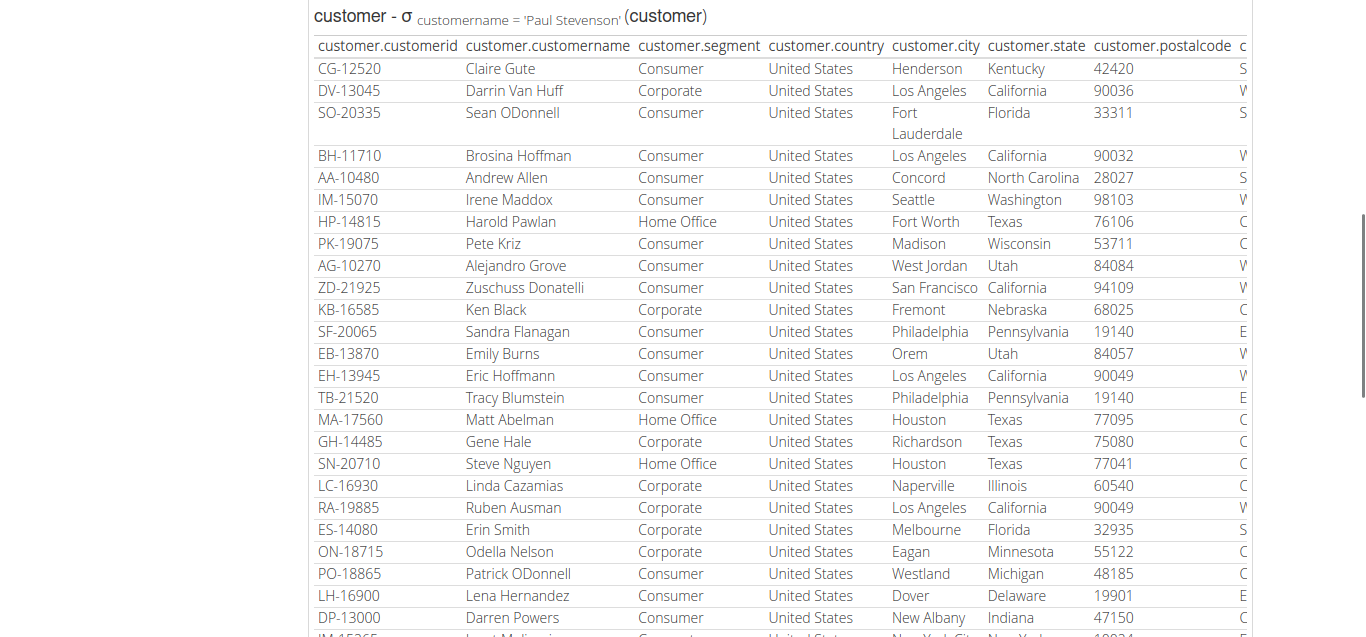
\includegraphics[scale=0.4]{assets/mantenimiento_datos-a.png}

			\item [b.] Borrar todas las ordenes de la ciudad de \texttt{Utah} que tengan artículos
				de la subcategoría \texttt{Tables}.\\
				Consulta:\\
				$A = \pi_{CustomerID} (\sigma_{State = 'Utah'} Customer)$\\
				$B = \pi_{ProductID} (\sigma_{Subcategory = 'Tables'} Products)$\\
				$Orders1 = Orders - (Orders \bowtie A \bowtie B)$\\

				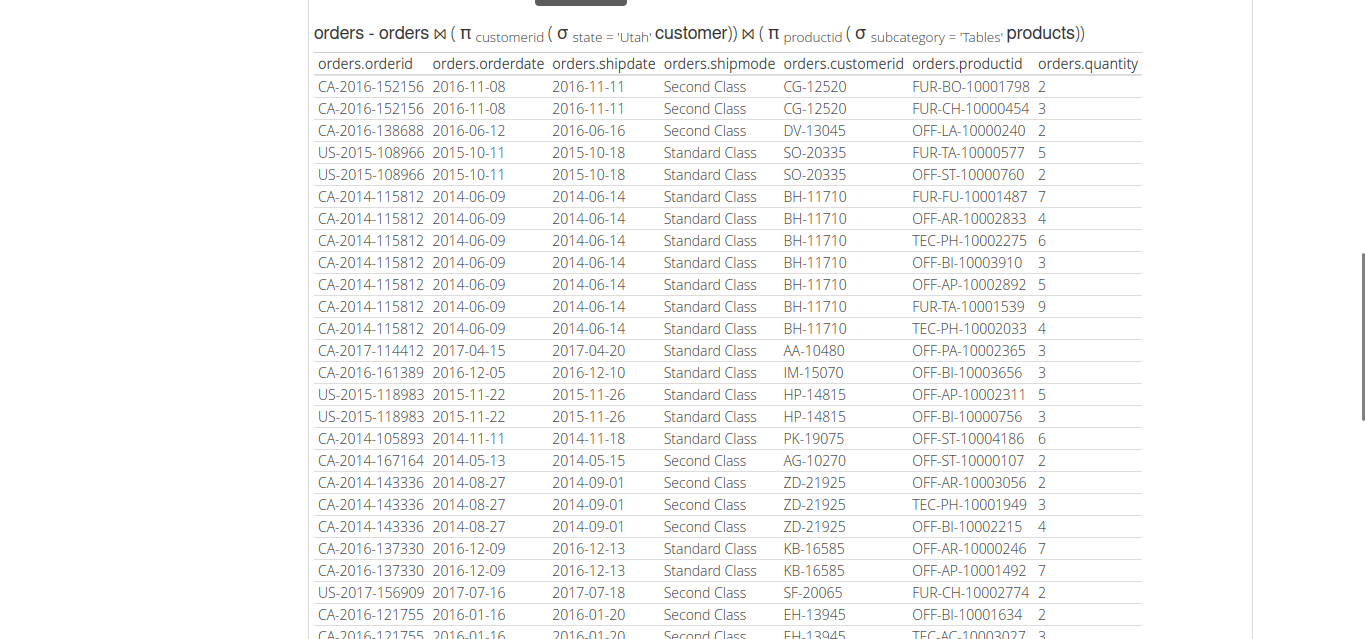
\includegraphics[scale=0.4]{assets/mantenimiento_datos-b.png}

			\item [c.] La clienta \texttt{Lena Cacioppo} compró un producto de cada subcategoría de \texttt{Furniture}.
				Deberás elegir los productos que desees e indicar como parte de esta consulta,
				la información que se agregará en cada caso.\\

				Elegimos un producto de cada categoría al azar y obtuvimos su id. Luego construimos una
				relación en línea (juntándola con la id de la clienta) y la unimos a Orders.\\

				\pagebreak
				Información agregada: (Orders)\\

				\begin{table}[h!]
				\begin{tabular}{|l|l|l|l|l|l|l|}
					\hline
					OrderID				&OrderDate	&ShipDate	&ShipMode		&CustomerID	&ProductID			&Quantity\\
					\hline
					'US-2022-000001'	&2022-11-06	&2022-11-08	&First Class	&LC-16870	&FUR-BO-10001798	&3\\
					'US-2022-000002'	&2022-11-06	&2022-11-08	&First Class	&LC-16870	&OFF-LA-10000240	&3\\
					'US-2022-000003'	&2022-11-06	&2022-11-08	&First Class	&LC-16870	&TEC-PH-10001949	&3\\
					\hline
				\end{tabular}
				\end{table}

				La consulta quedo:\\
				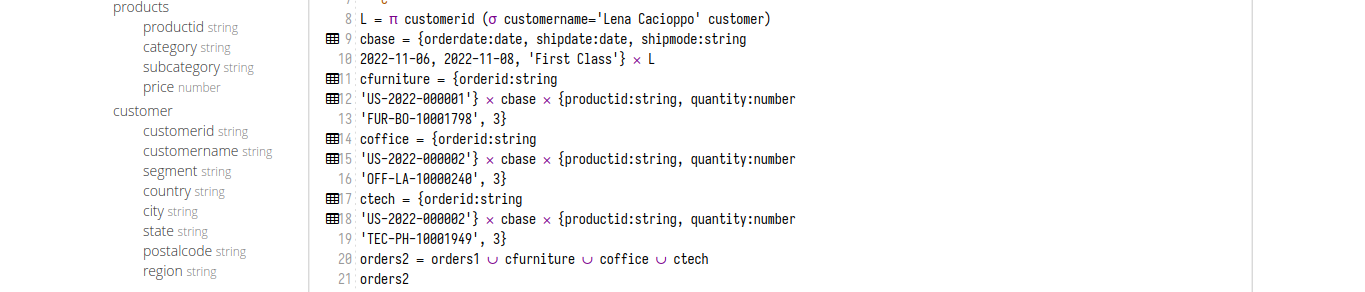
\includegraphics[scale=0.4]{assets/mantenimiento_datos-c1.png}

				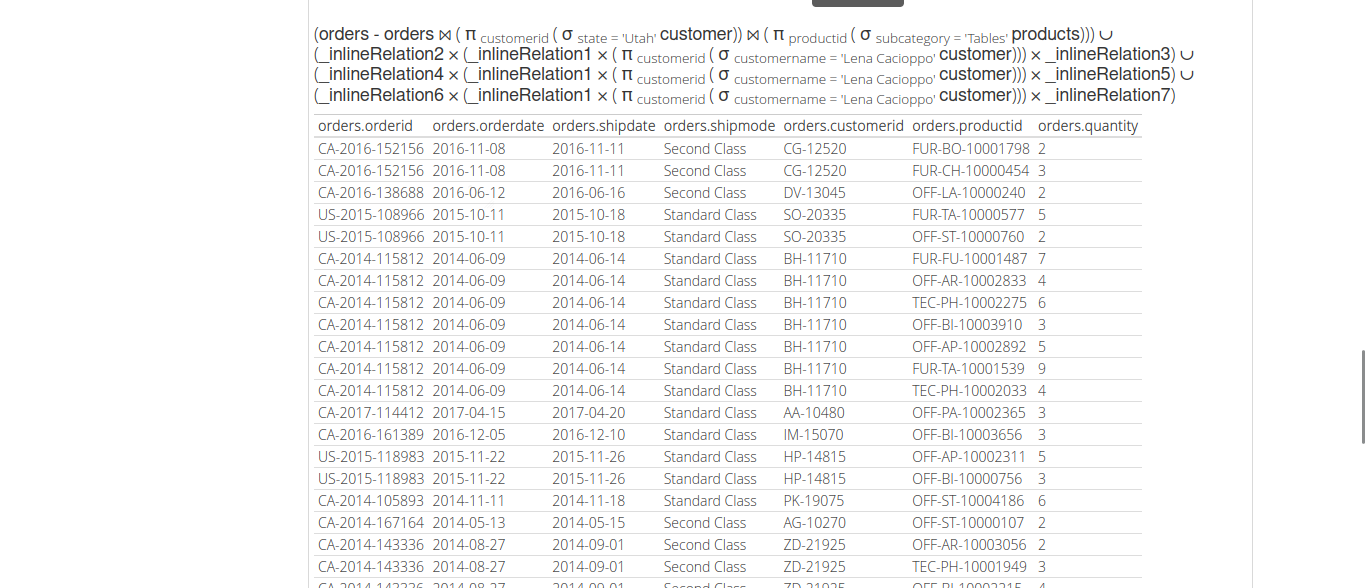
\includegraphics[scale=0.4]{assets/mantenimiento_datos-c2.png}

			\item [d.] Aumentar los precios de productos de la subcategoría \texttt{Phones} en un \texttt{8\%}.\\
				Consulta:\\
				$A = \sigma_{Subcategory = 'Phones'} (Products)$\\
				$U = \pi_{ProductID, Category, Subcategory, price\leftarrow price * 1.08} A$\\
				$Products = (Products - A) \cup U$\\

				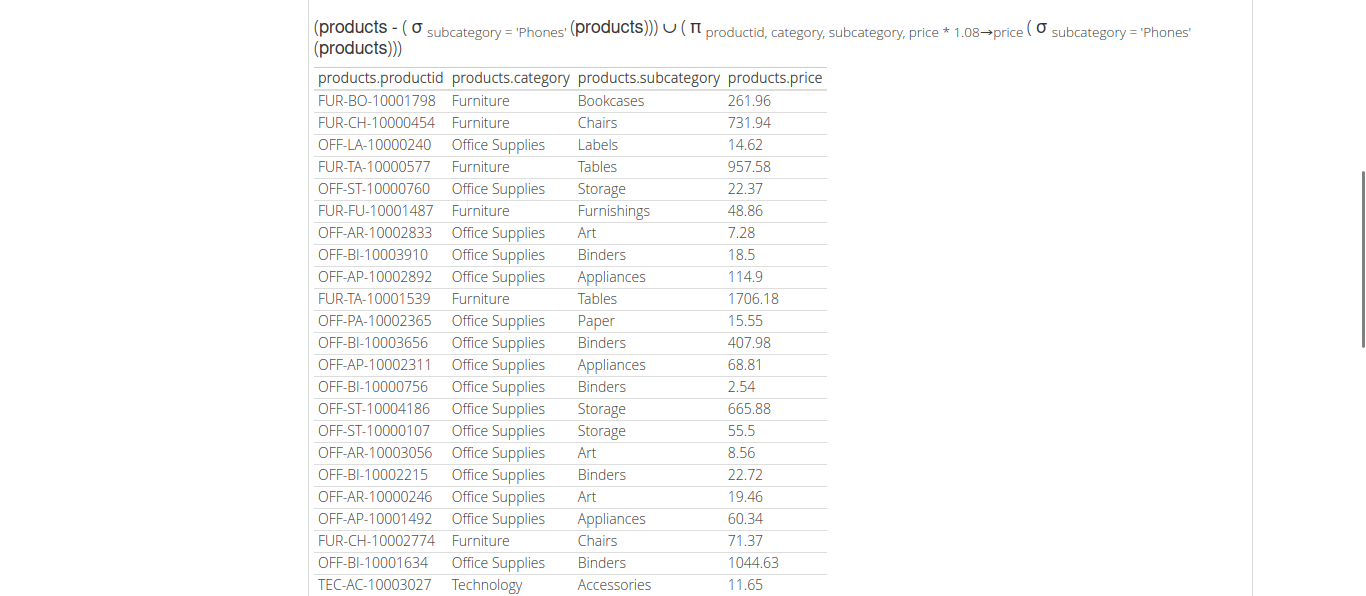
\includegraphics[scale=0.4]{assets/mantenimiento_datos-d.png}

				\pagebreak
			\item [e.] Disminuir \texttt{8\%} los precios de los productos de la categoría \texttt{Furniture}
				cuyo precio sea de \texttt{\$600} a \texttt{\$900}.
				Aumentar en un \texttt{5\%} los precios de los productos de
				la categoría Technology y subcategoría Machines.\\

				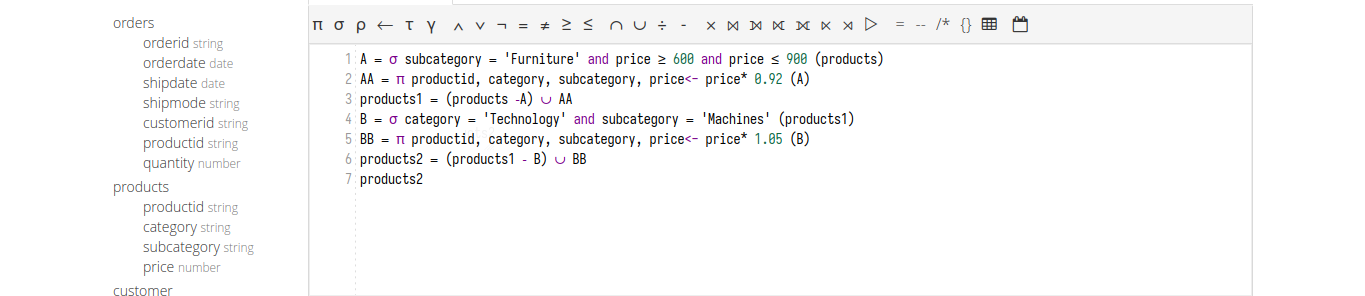
\includegraphics[scale=0.4]{assets/mantenimiento_datos-e1.png}

				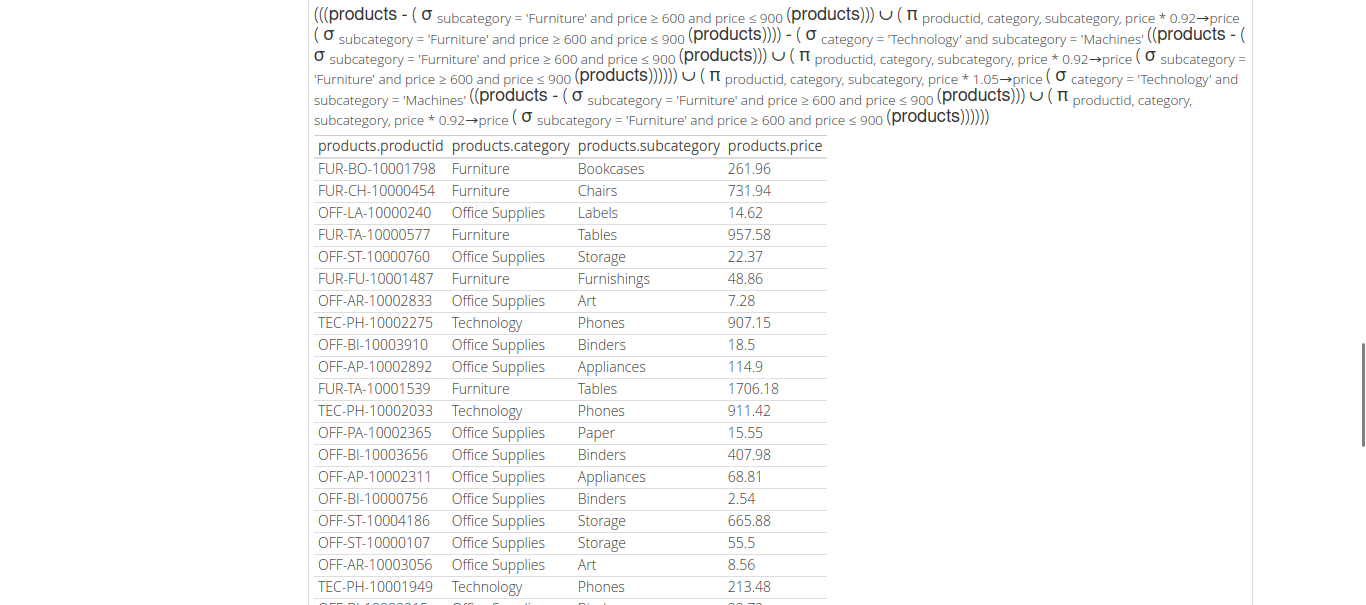
\includegraphics[scale=0.4]{assets/mantenimiento_datos-e2.png}
		\end{enumerate}
\end{enumerate}
\end{document}

